% Uncomment this to make slides with overlays:
%\documentclass[slides]{beamer}

%% Uncomment these (but comment the above \documentclass line) to make handouts:
\documentclass[handout]{beamer}

% Uncomment these to have more than one slide per page
\usepackage{pgfpages}
\pgfpagesuselayout{2 on 1}[border shrink=5mm]
\pgfpageslogicalpageoptions{1}{border code=\pgfusepath{stroke}}
\pgfpageslogicalpageoptions{2}{border code=\pgfusepath{stroke}}

\usepackage[]{graphicx, color, hyperref}

\mode<presentation>
{
	%\usetheme[secheader]{Boadilla}
	%\usecolortheme[rgb={.835, .102,.169}]{structure}  
	\usetheme[width= 0cm]{Goettingen}
	%\setbeamercovered{transparent}
}
\setbeamertemplate{navigation symbols}{}
\setbeamertemplate{footline}[frame number]

\definecolor{blue2}{rgb}{0.278,0.278,0.729} 
\newcommand{\blue}[1]{\textcolor{blue2}{#1}}
\newcommand{\white}[1]{\textcolor{white}{#1}}
\newcommand{\red}[1]{\textcolor{red}{#1}}
\newcommand{\xbar}{\overline{x}}
\newcommand{\ybar}{\overline{y}}
\newcommand{\phat}{\widehat{p}}
\newcommand{\prob}{\mbox{Pr}}
\newcommand{\E}{\mathbb{E}}
\newcommand{\Var}{\mbox{Var}}
\newcommand{\cp}{\oplus}
\newcommand{\cm}{\circleddash}

\title{Lecture 9: Normal Approximation}
\author{Chapter 3.2}
\date{}


\begin{document}
%------------------------------------------------------------------------------
\begin{frame}
\titlepage
\end{frame}
%------------------------------------------------------------------------------


%------------------------------------------------------------------------------
\begin{frame}[fragile]
\frametitle{Goals for Today}

\begin{itemize}
\item Discuss how to find \%'iles for negative values of $z$
\item Examples
\item Evaluating how ``normal'' certain data are.  
\end{itemize}

\end{frame}
%------------------------------------------------------------------------------


%------------------------------------------------------------------------------
\begin{frame}
\frametitle{Solving Normal Questions}
Whenever solving questions of this sort \blue{ALWAYS} draw a rough picture first and keep in mind:
\begin{enumerate}
\item The normal distribution/curve is \blue{symmetric}
\item The total area under the curve is 1
\end{enumerate}

\end{frame}
%------------------------------------------------------------------------------


%------------------------------------------------------------------------------
\begin{frame}
\frametitle{Normal Probability Tables}
Alternatively, whereas 
\begin{itemize}
\item table on P.409 gives areas to the left of positive values of $z$.
\item table on P.408 gives areas to the left of negative values of $z$.
\end{itemize}

\vspace{0.5cm}
I'm only going to give you P.409 table for exams.

\end{frame}
%------------------------------------------------------------------------------


%------------------------------------------------------------------------------
\begin{frame}
\frametitle{Speeding on I-5}
The distribution of passenger vehicle speeds traveling on Interstate 5 Freeway (I-5) in California is nearly normal with a mean of 72.6 mph and a standard deviation of 4.78 mph.

\vspace{0.25cm}

\begin{enumerate}
\item[a)] What percent of passenger vehicles travel slower than 80 mph?
\item[b)] What percent of passenger vehicles travel between 60 and 80 mph?
\item[c)] How fast to do the fastest 5\% of passenger vehicles travel?
\item[d)] The speed limit on this stretch of the I-5 is 70 mph. Approximate what percentage of
the passenger vehicles travel above the speed limit on this stretch of the I-5.
\end{enumerate}

\end{frame}
%------------------------------------------------------------------------------


%------------------------------------------------------------------------------
\begin{frame}
\frametitle{Speeding on I-5}
a) What percent of passenger vehicles travel slower than 80 mph?

\vspace{7cm}

\end{frame}
%------------------------------------------------------------------------------


%------------------------------------------------------------------------------
\begin{frame}
\frametitle{Speeding on I-5}
b) What percent of passenger vehicles travel between 60 and 80 mph?

\vspace{7cm}

\end{frame}
%------------------------------------------------------------------------------


%------------------------------------------------------------------------------
\begin{frame}
\frametitle{Speeding on I-5}
c) How fast to do the fastest 5\% of passenger vehicles travel?

\vspace{7cm}

\end{frame}
%------------------------------------------------------------------------------


%------------------------------------------------------------------------------
\begin{frame}
\frametitle{Speeding on I-5}
d) The speed limit on this stretch of the I-5 is 70 mph. Approximate what percentage of
the passenger vehicles travel above the speed limit on this stretch of the I-5.

\vspace{7cm}

\end{frame}
%------------------------------------------------------------------------------


%------------------------------------------------------------------------------
\begin{frame}
\frametitle{Switching Gears: Normal Approximation}

Although we stated that many processes in the physical world look bell-shaped, i.e. roughly normal, we must keep in mind that this is an \blue{approximation}.  

\vspace{0.5cm}

\pause\blue{Question}: How do we verify normality?

\end{frame}
%%------------------------------------------------------------------------------


%%------------------------------------------------------------------------------
%\begin{frame}
%\frametitle{Normal Approximation}
%
%Consider the MLB salary data histogram:
%
%\begin{center}
%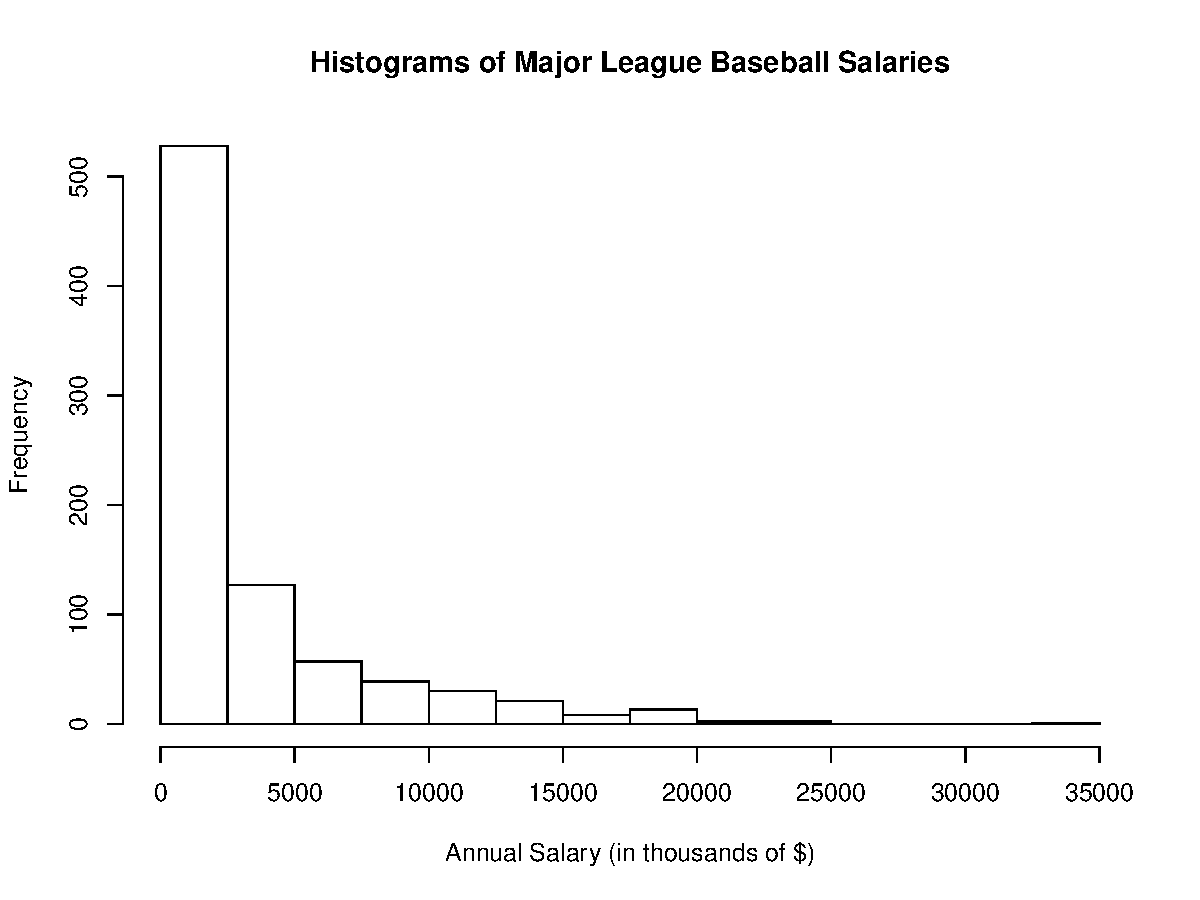
\includegraphics[width=7cm]{figure/MLB.pdf}
%\end{center}
%
%\end{frame}
%%------------------------------------------------------------------------------


%------------------------------------------------------------------------------
\begin{frame}
\frametitle{Normal Approximation}

What about these ones?  How well do the histograms fit to the normal curve?

\begin{center}
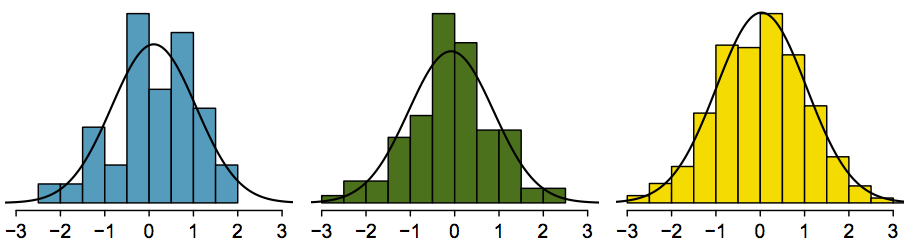
\includegraphics[width=\textwidth]{figure/normal_hist.png}
\end{center}

\end{frame}
%------------------------------------------------------------------------------


%------------------------------------------------------------------------------
\begin{frame}
\frametitle{Normal Probability Plots}
\blue{Normal probability plots} (AKA quantile-quantile plots AKA QQ-plots) are a method for visually displaying how well data fit a normal curve.

\vspace{0.75cm}

\pause The $k^{\mbox{th}}$ \blue{$q-quantile$} is the value such that proportion $\frac{k}{q}$ of the observations fall below it.  So 
\begin{itemize}
\pause\item The 4-quantiles are the \blue{quartiles}.\\
%Ex: the $k=2^{\mbox{nd}}$ 4-quantile is just the median.  
\pause\item The 100-quantiles are the \blue{percentiles}.\\
%Ex: the $k=76^{\mbox{th}}$ 100-quantile is just the 76th percentile
\end{itemize}

\end{frame}
%------------------------------------------------------------------------------


%------------------------------------------------------------------------------
\begin{frame}
\frametitle{Normal Probability Plots}
A normal probability plot compares:

\begin{itemize}
\item The \blue{observed} quantiles of a data set (on the $y$-axis)
\item The \blue{theoretical} quantiles that are \blue{exactly} normal (on the $x$-axis)
\end{itemize}

\pause\vspace{0.5cm}

The more ``normal'' the data is, the better the fit.  

\end{frame}
%------------------------------------------------------------------------------


%------------------------------------------------------------------------------
\begin{frame}
\frametitle{Normal Probability Plots}
\begin{center}
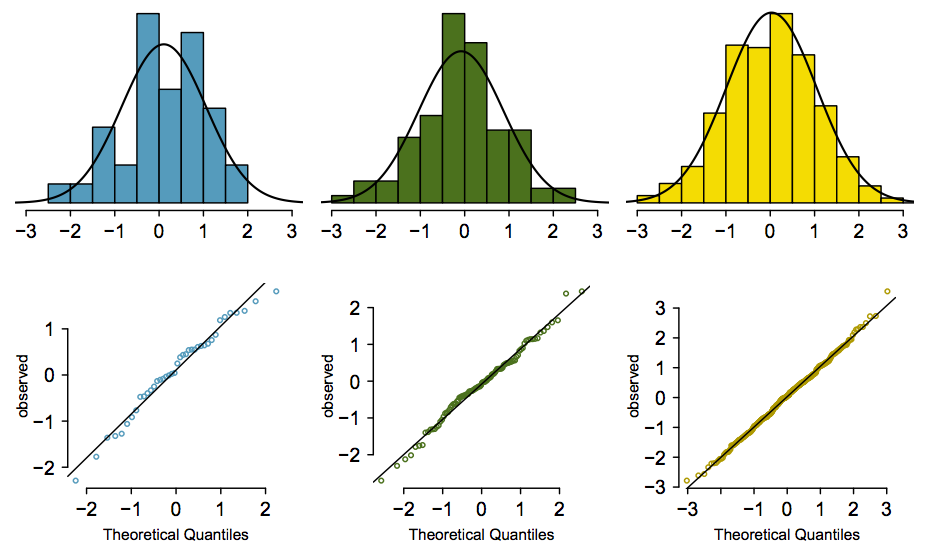
\includegraphics[width=\textwidth]{figure/normal_hist2.png}
\end{center}
\end{frame}
%------------------------------------------------------------------------------


%%library(openintro)
%%data(MLB)
%%pdf("./4.2 Normal Approximation/MLB_qqplot.pdf", width=6, height=6)
%%qqnorm(MLB$salary)
%%qqline(MLB$salary, lwd=1.5)
%%dev.off()
%%------------------------------------------------------------------------------
%\begin{frame}[fragile]
%\frametitle{MLB Salary Normal Probability Plot}
%
%\begin{center}
%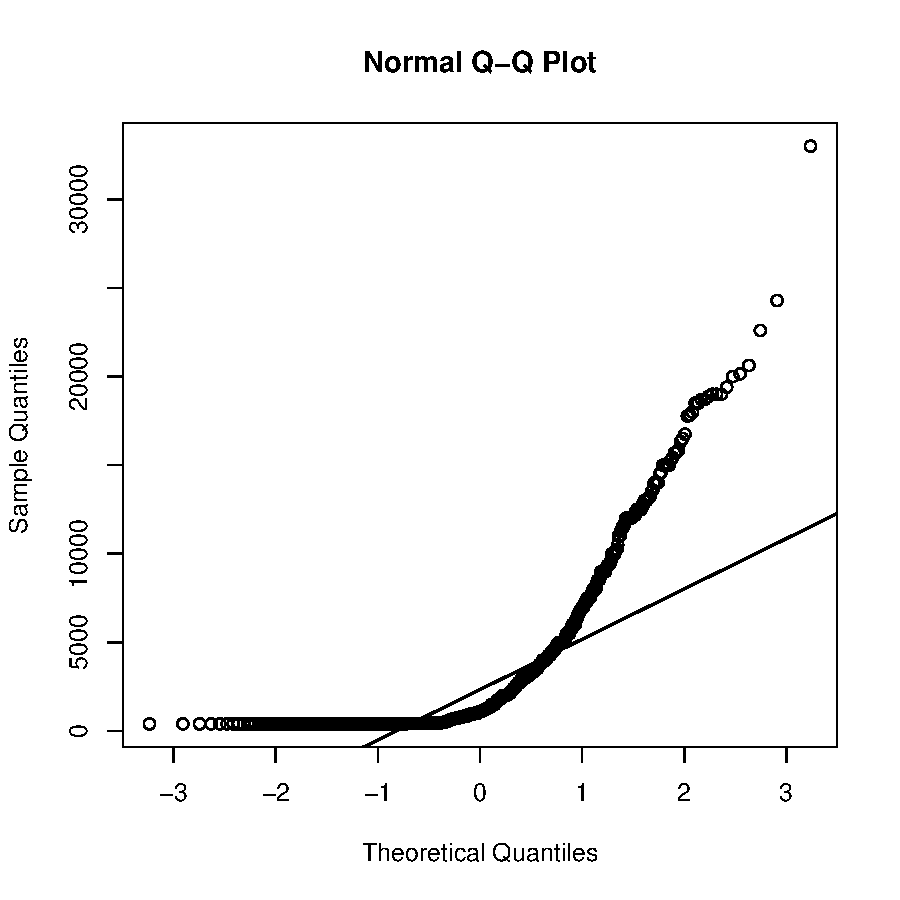
\includegraphics[width=5cm]{figure/MLB_qqplot.pdf}
%\end{center}
%\begin{verbatim}
%library(openintro)
%data(MLB)
%qqnorm(MLB$salary)
%qqline(MLB$salary)
%\end{verbatim}
%\end{frame}
%%------------------------------------------------------------------------------


%------------------------------------------------------------------------------
\begin{frame}[fragile]
\frametitle{Next Time}

\begin{itemize}
\item Introduce some of the more useful other distributions: Bernoulli, Geometric, Binomial, and Poisson
\end{itemize}


\end{frame}
%------------------------------------------------------------------------------


\end{document}










